\documentclass[11pt, oneside]{article} 
\usepackage{geometry}
\geometry{letterpaper} 
\usepackage{graphicx}
	
\usepackage{amssymb}
\usepackage{amsmath}
\usepackage{parskip}
\usepackage{color}
\usepackage{hyperref}

\graphicspath{{/Users/telliott_admin/Dropbox/Tex/png/}}
% \begin{center} 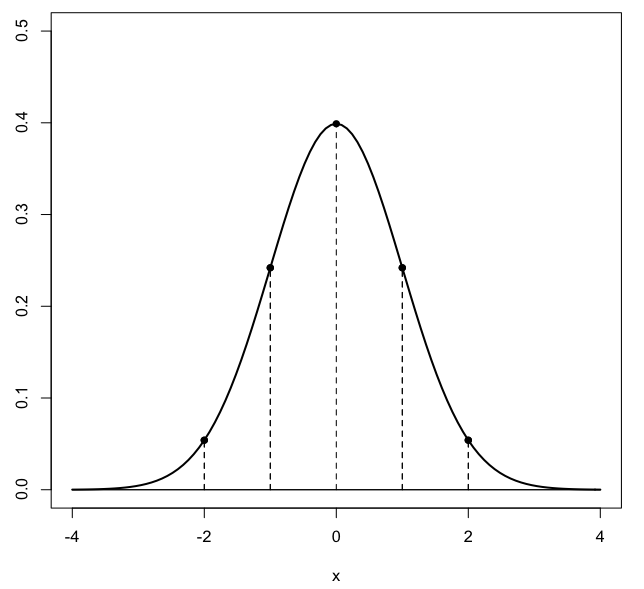
\includegraphics [scale=0.4] {gauss3.png} \end{center}

\title{Parametric equations}
\date{}

\begin{document}
\maketitle
\Large

\label{sec:Parametric_equations}

Suppose we are working in $\mathbb{R}^2$.  Consider two points $P = (x_1,y_1)$ and $Q = (x_2, y_2)$.  The vector $\mathbf{v}$ which goes in the direction $PQ$ can be obtained as
\[ \mathbf{v} = \langle \ x_2 - x_1, y_2 - y_1 \rangle \]

Written like that as just $\mathbf{v}$ by itself, the default would be that we consider that vector to lie with its tail at the origin.  Multiplying by a real number $t$ will extend the vector to any point lying on the line with slope
\[ m = \frac{y_2 - y_1}{x_2 - x_1} \]
that goes through the origin.  

If $t < 0$ then the vector goes backward.

To start from some other position, add the vector which extends to that point.  The position vector is commonly called $\mathbf{r}$.  So the complete specification of a line in $\mathbb{R}^2$ would be something like:
\[ l = \mathbf{r} + t \mathbf{v} \]
This is called the \emph{parametric} representation of the line.

As a second example, consider a circle of radius $R$ with its center at the origin.  We can write the equation of this circle in several ways.  In Cartesian coordinates:
\[ x^2 + y^2 = R^2 \]
In polar coordinates:
\[ r = R \]
or parametrically
\[ x = R \cos \theta \]
\[ y = R \sin \theta \]
where $\theta$ takes on values in the interval $[0, 2\pi]$.

With the appropriate units for $t$, we can write
\[ x = R \cos t \]
\[ y = R \sin t \]
where $t$ is often understood to be the time, although it doesn't have to be.  (Alternatively, we might use the time and an angular velocity $\omega$ in the combination as $\omega t$).

We can write something equivalent using only one variable, for the position vector
\[ \mathbf{r}(t) = \langle \ R \cos t, R \sin t \rangle = R \ \langle \cos t, \sin t \rangle  \]

In three dimensions, we just add another component to $\mathbf{r}$ for $z$.  Perhaps
\[ \mathbf{r}(t) =  \ \langle \cos t, \sin t, t  \rangle  \]
which traces out a spiral whose shadow in the $xy$-plane is the unit circle.

We can do calculus with vector functions of this type:  both differentiating and integrating.

The rule is simple:  the dimensions are independent.  We differentiate each one separately.  For example:
\[ \mathbf{r} =  \ \langle \cos t, \sin t \rangle \]
\[ \frac{d}{dt} \ \mathbf{r} =  \ \langle - \sin t, \cos t \rangle \]
but
\[ \frac{d \mathbf{r}}{dt} = \mathbf{\dot{r}} = \mathbf{v} \]
the time-derivative of position is velocity.

So, we observe that, for motion on the unit circle, the velocity is perpendicular to the position vector because
\[ \mathbf{r} \cdot \mathbf{v} =  \langle \ \cos t, \sin t \rangle \cdot \langle -\sin t, \cos t \rangle = 0 \]

By the same logic the acceleration is
\[ \mathbf{a} = \frac{d \mathbf{v}}{dt} = \mathbf{\ddot{r}} = \ \langle -\cos t, -\sin t \rangle  \]
The acceleration vector $\mathbf{a}$ points in the same direction as the position vector $\mathbf{r}$, with opposite sign.

Observe that the magnitude of the velocity vector is
\[ |\mathbf{v}| = \sqrt{\sin^2 t + \cos^2 t} = 1 \]
This magnitude of $\mathbf{v}$ is unchanging in time.  So on the circle, there is acceleration even though the speed is constant

\subsection*{tangent and normal}

We observe that the velocity vector at a point  is tangent to the curve.  So, if we need a unit tangent vector
\[ \mathbf{\hat{T}} = \frac{\mathbf{v}}{|\mathbf{v}|} \]
All of these are functions of $t$.  We could have written:
\[ \mathbf{\hat{T}}(t) = \frac{\mathbf{v}(t)}{|\mathbf{v}(t) |} \]
But we resist the urge to do that.

The normal vector $\mathbf{\hat{n}}$ to the curve is perpendicular to $\mathbf{\hat{T}}$.  We construct $\mathbf{\hat{n}}$ in the usual way, by taking the $x$ and $y$ components of $\mathbf{\hat{T}}$ and writing:
\[ \mathbf{\hat{n}} = \ \langle - y, x \rangle \]
or $\langle y, -x \rangle$.  In either case, the dot product with $\mathbf{v}$ will be zero.

For an ellipse, we can parametrize like this:
\[ \mathbf{r} = \ \langle a \cos t, b \sin t \rangle \]
\[ \mathbf{v} = \ \langle -a \sin t, b \cos t \rangle \]
Now, it is no longer true that the tangent and the position vector are orthogonal.  The ellipse is more interesting than the circle in this respect, as we will see.

I would just mention that for a surface, we need two variables in the parametrization.  For example, to parametrize the surface of the sphere, we might use the polar angle $\phi$ and the radial angle $\theta$.  Any position on the globe can be specified with its longitude and latitude.  We'll see a lot more about this as well.

\subsection*{time-derivative of products}
As we mentioned above, to take the derivative with respect to the parameter (such as time), we just go through each component of a vector
\[ \mathbf{r} = \langle x, y, z \rangle \]
\[ \frac{d \mathbf{r}}{dt} =  \langle \frac{dx}{dt}, \frac{dy}{dt}, \frac{dz}{dt} \rangle \]

The question arises, what about products?  Is there a product rule for vectors?  Here's an example
\[ \frac{d}{dt} \ \mathbf{r} \cdot \mathbf{v} \]
It turns out that there is.
\[ \frac{d}{dt} \ \mathbf{r} \cdot \mathbf{v} = \frac{d \mathbf{r}}{dt} \cdot \mathbf{v} + \mathbf{r} \cdot \frac{d \mathbf{v}}{dt}  \]
The reason is that the individual components of the dot product are simple functions of $t$, and our rule is to differentiate one component at a time.

Let's use Newton's dot notation for $d/dt$:
\[ \mathbf{r} = \langle x, y, z\rangle \]
\[ \mathbf{\dot{r}} = \mathbf{v} = \langle \dot{x}, \dot{y}, \dot{z} \rangle \]
\[ \mathbf{r} \cdot \mathbf{\dot{r}}  = x \dot{x} + y \dot{y} + z \dot{z} \]
The derivative is
\[ \frac{d}{dt} \mathbf{r} \cdot \mathbf{\dot{r}}  = \frac{d}{dt} ( x \dot{x} + y \dot{y} + z \dot{z} ) \]
\[ = \dot{x} \dot{x} + x \ddot{x} + \dot{y} \dot{y} + y \ddot{y} + \dot{z} \dot{z} + z \ddot{z}  \]
\[ = \dot{x} \dot{x} + \dot{y} \dot{y} + \dot{z} \dot{z} + x \ddot{x}  + y \ddot{y} + z \ddot{z}  \]
\[ =  \mathbf{\dot{r}} \cdot \mathbf{\dot{r}} +  \mathbf{r} \cdot \mathbf{\ddot{r}} \]

The same is true of the cross-product.  The torque is $\mathbf{F} \times \mathbf{r}$  Let's take the derivative:
\[ \frac{d}{dt} \ [ \ \mathbf{F} \times \mathbf{r} \ ] \ = \]
Let's write $\mathbf{F} = \langle M,N,P \rangle$, then the cross-product gives a vector with components
\[ \ [ \ N z - P y \ ] \ \mathbf{\hat{i}} + \ [ \ P x - M z \ ] \ \mathbf{\hat{j}} + \ [ \ M y - N x \ ] \ \mathbf{\hat{k}} \]
where both $M,N,P$ and $x,y,z$ are \emph{functions} of time.

The time derivative is obtained by the product rule.  Again, I will use dots, and here we separate the components onto different lines:
\[ \ [ \ \dot{N} z + N \dot{z} - \dot{P} y - P \dot{y} \ ] \ \mathbf{\hat{i}} + \]
\[ + \  [ \ \dot{P} x + P \dot{x} - \dot{M} z - M \dot{z} \ ] \ \mathbf{\hat{j}} + \]
\[ +  \ [ \ \dot{M} y + M \dot{y} - \dot{N} x - N \dot{x} \ ] \ \mathbf{\hat{k}} \]

but this is just two different cross-products added together.  The first one is
\[ \ [ \ \dot{N} z - \dot{P} y \ ] \ \mathbf{\hat{i}} + \  [ \ \dot{P} x - \dot{M} z \ ] \ \mathbf{\hat{j}} +  \ [ \ \dot{M} y - \dot{N} x \ ] \ \mathbf{\hat{k}} \]
\[ = \mathbf{\dot{F}} \times \mathbf{r} \]

and the second is:
\[ \ [ \  N \dot{z}  - P \dot{y} \ ] \ \mathbf{\hat{i}} + \  [ \ P \dot{x} - M \dot{z} \ ] \ \mathbf{\hat{j}} +  \ [ \ M \dot{y} - N \dot{x} \ ] \ \mathbf{\hat{k}} \]
\[ = \mathbf{F} \times \mathbf{\dot{r}} \]

Putting it all together
\[ \frac{d}{dt} \ [ \ \mathbf{F} \times \mathbf{r} \ ] \ = \mathbf{\dot{F}} \times \mathbf{r} + \mathbf{F} \times \mathbf{\dot{r}} \]

The product rule for differentiation holds for both the dot product and the cross-product.


\end{document}